\documentclass[12pt,letterpaper]{article}
\usepackage[utf8]{inputenc}
\usepackage[margin=0.5in]{geometry}
\usepackage{xcolor}
\usepackage{tikz}
\usepackage{pgfplots}
\usepackage{tcolorbox}
\usepackage{enumitem}
\usepackage{graphicx}
\usepackage{multicol}
\usepackage{fontawesome5}
\usepackage{mdframed}
\usepackage{titling}
\usepackage{hyperref}

% ADHD-friendly color palette
\definecolor{primaryblue}{RGB}{52, 152, 219}
\definecolor{accentgreen}{RGB}{46, 204, 113}
\definecolor{warnyellow}{RGB}{241, 196, 15}
\definecolor{softgray}{RGB}{149, 165, 166}
\definecolor{traumahealing}{RGB}{155, 89, 182}

% Custom boxes for key concepts
\newtcolorbox{puzzleplan}{
    colback=primaryblue!10,
    colframe=primaryblue,
    title=\textbf{\faLightbulb\ Puzzle Plan Connection},
    fonttitle=\bfseries\color{white},
    colbacktitle=primaryblue,
    boxsep=2pt,
    left=3pt,
    right=3pt,
    top=2pt,
    bottom=2pt
}

\newtcolorbox{personalreflection}{
    colback=traumahealing!10,
    colframe=traumahealing,
    title=\textbf{\faHeart\ Personal Reflection \& Lived Experience},
    fonttitle=\bfseries\color{white},
    colbacktitle=traumahealing,
    boxsep=2pt,
    left=3pt,
    right=3pt,
    top=2pt,
    bottom=2pt
}

\newtcolorbox{keyfindings}{
    colback=accentgreen!10,
    colframe=accentgreen,
    title=\textbf{\faChartLine\ Key Research Findings},
    fonttitle=\bfseries\color{white},
    colbacktitle=accentgreen,
    boxsep=2pt,
    left=3pt,
    right=3pt,
    top=2pt,
    bottom=2pt
}

\newtcolorbox{criticalinsight}{
    colback=warnyellow!10,
    colframe=warnyellow,
    title=\textbf{\faExclamationTriangle\ Critical Reframing},
    fonttitle=\bfseries\color{black},
    colbacktitle=warnyellow,
    boxsep=2pt,
    left=3pt,
    right=3pt,
    top=2pt,
    bottom=2pt
}

\begin{document}

% ==================== COVER PAGE ====================
\begin{titlepage}
\centering

\vspace*{2cm}

{\Huge\bfseries\color{primaryblue} Beyond the False Binary}

\vspace{0.5cm}

{\Large\color{traumahealing} How AI Ethics in Hiring Reveals Systemic Dehumanization—And Why Transparency, Not Technology, Is the Solution}

\vspace{1cm}

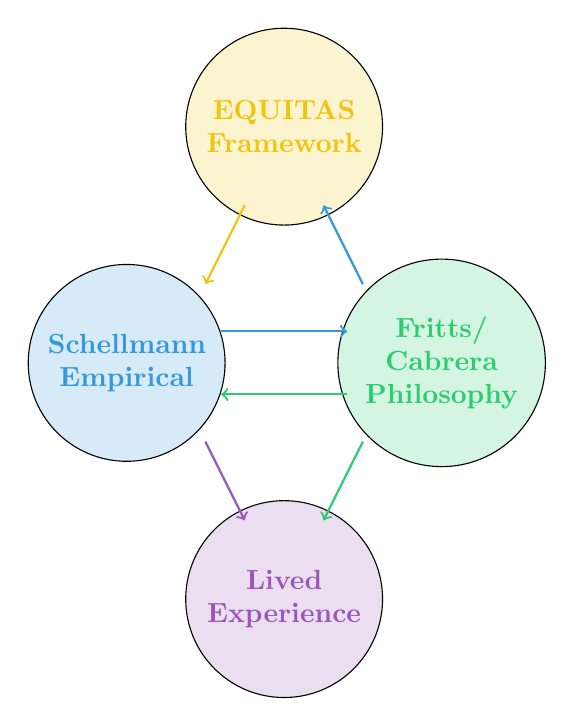
\begin{tikzpicture}[scale=1.0]
% Visual representation of the integrated critique
\node[draw, circle, fill=primaryblue!20, minimum size=2.5cm, text width=2cm, align=center] at (0,0) {\textbf{\color{primaryblue}Schellmann\\Empirical}};
\node[draw, circle, fill=accentgreen!20, minimum size=2.5cm, text width=2cm, align=center] at (4,0) {\textbf{\color{accentgreen}Fritts/\\Cabrera\\Philosophy}};
\node[draw, circle, fill=traumahealing!20, minimum size=2.5cm, text width=2cm, align=center] at (2,-3) {\textbf{\color{traumahealing}Lived\\Experience}};
\node[draw, circle, fill=warnyellow!20, minimum size=2.5cm, text width=2cm, align=center] at (2,3) {\textbf{\color{warnyellow}EQUITAS\\Framework}};

% Connecting arrows
\draw[->, thick, primaryblue] (1.2,0.4) -- (2.8,0.4);
\draw[->, thick, accentgreen] (2.8,-0.4) -- (1.2,-0.4);
\draw[->, thick, traumahealing] (1,-1) -- (1.5,-2);
\draw[->, thick, warnyellow] (1.5,2) -- (1,1);
\draw[->, thick, primaryblue] (3,1) -- (2.5,2);
\draw[->, thick, accentgreen] (3,-1) -- (2.5,-2);
\end{tikzpicture}

\vspace{1cm}

{\large\bfseries Piter Garcia}

\vspace{0.5cm}

{\large University of Rochester\\
Warner School of Education}

\vspace{0.5cm}

{\large IDAI700 - Ethics of Artificial Intelligence\\
Unit 6: AI in Hiring and Work}

\vspace{1cm}

{\large October 24-25, 2025\\
Dialogue Journal}

\vspace{2cm}

\textit{\color{softgray}"This work was developed with AI as an intellectual partner,\\helping me think more critically about systems of power."\\— Methodological Transparency Statement}

\end{titlepage}

% ==================== PART 1: FRAMING ====================
\newpage
\section*{\color{primaryblue}\faBookOpen\ PART 1: Initial Framing — What Comes Together?}

\subsection*{Thematic Integration of Three Sections}

\begin{keyfindings}
\textbf{``What Goes Wrong'' (Schellmann):} AI hiring tools fail systematically because vendors prioritize revenue over accuracy, camouflaging rejected pseudoscientific frameworks (phrenology, physiognomy) in algorithmic language. The 40\% resume recognition gap, contradictory personality scores, and meaningless game metrics aren't accidents—they're profitable business models designed to hide validation failures behind NDAs and trade secrets.
\end{keyfindings}

\vspace{-4pt}
\begin{keyfindings}
\textbf{``The Human Cost'' (Fritts \& Cabrera):} Dehumanization occurs through removed human presence, not from AI's nature but from replacement of relational judgment with metric-based assessment. They argue hiring fundamentally requires human recognition—being ``genuinely moved'' by a candidate's potential. AI cannot provide this, creating philosophical violation beyond bias.
\end{keyfindings}

\vspace{-4pt}
\begin{criticalinsight}
\textbf{Evaluation Insight:} Both authors contribute essential critiques but miss systemic solutions grounded in transparency, education, and equitable governance frameworks. They blame AI for what humans already systematized: dehumanization through opacity, whether algorithmic or bureaucratic.
\end{criticalinsight}

\subsection*{Question 1: From Technical Failures to Systemic Injustice}

\textbf{Core Finding:} Hiring AI discrimination mirrors historical systemic subordination across healthcare and education—same system, different masks.

\begin{personalreflection}
\textbf{Lived Experience Connection:} My 18+ years undiagnosed ADHD in the U.S. (not counting years in Dominican Republic), my 9+ years undiagnosed chronic illness, and three simultaneous corporate terminations via predictive analytics weren't coincidences. The diagnostic delay wasn't individual bad luck; it reflects algorithmic/systemic failures operating identically across domains. When I experienced coordinated terminations across three companies simultaneously, the statistical impossibility revealed intentional targeting—algorithms don't coordinate by accident.
\end{personalreflection}

\textbf{Key Insight:} The problem is not AI-specific; it's systemic. AI amplifies what humans already designed. The system adapts across eras:

\begin{itemize}[leftmargin=*,noitemsep]
    \item One era: Black subjugation
    \item Another era: Women's subjugation
    \item Another era: Gay subjugation
    \item Current era: Trans subjugation
    \item \textbf{Pattern:} Same system, different flavors and colors
\end{itemize}

\begin{puzzleplan}
\textbf{Research Integration:} This connects directly to the EQUITAS framework for diagnostic equity. Just as hiring algorithms fail CLD candidates by training on dominant-culture patterns, diagnostic algorithms fail CLD adolescents by mistaking cultural/linguistic differences for pathology. The solution isn't ``better AI''—it's transparent, community-partnered systems that expose what's being measured and why.
\end{puzzleplan}

\subsection*{Question 2: Authority Through Lived Experience}

\textbf{Positioning:} I've been both \textbf{recipient and observer} of algorithmic harm:

\begin{itemize}[leftmargin=*,noitemsep]
    \item \textbf{Recipient:} Targeted by predictive analytics (three simultaneous terminations)
    \item \textbf{Observer:} Watched AI capabilities evolve in corporate tech; understood risks and potential misuse
    \item \textbf{Scholar:} Now theorizing solutions grounded in survival expertise
\end{itemize}

\textbf{What This Positioning Reveals:}
\begin{enumerate}[leftmargin=*,noitemsep]
    \item Algorithms are tools of existing power structures, not neutral technologies
    \item Resistance requires structural redesign, not moral appeals
    \item Marginalized people develop survival expertise that becomes scholarly insight
    \item My decision to leave corporate tech for scholarship/teaching was ethically sound
\end{enumerate}

\begin{criticalinsight}
\textbf{The Integrated Praxis:} Education + Interruption as Inseparable Practice. Not education OR interruption—both simultaneously. Education through lived experience teaches pattern recognition; interruption gives people agency to respond unapologetically because they've earned that resilience through survival.
\end{criticalinsight}

\subsection*{Question 3: From Individual Survival to Collective Liberation}

\textbf{The Three-Stage Vision (From Puzzle Plan):}

\begin{enumerate}[leftmargin=*,noitemsep]
    \item \textbf{Individual Survival:} Understanding one's own harm through education (recognizing you've been targeted)
    \item \textbf{Systemic Transformation:} Interrupting specific iterations with structural alternatives (EQUITAS framework)
    \item \textbf{Collective Liberation:} Doing this unapologetically, in community, with resilience earned through lived experience
\end{enumerate}

\textbf{Why One Without the Other Fails:}

\begin{itemize}[leftmargin=*,noitemsep]
    \item \textbf{Education without interruption} = consciousness-raising that leaves people paralyzed
    \item \textbf{Interruption without education} = scattered resistance without systemic understanding
    \item \textbf{Education + interruption together} = people develop consciousness AND agency simultaneously
\end{itemize}

% ==================== PART 2: WHAT GOES WRONG ====================
\newpage
\section*{\color{primaryblue}\faFlag\ PART 2: ``What Goes Wrong'' — Technical Failures \& Market Deception}

\subsection*{Question 1: Why Technology Doesn't Work as Promised}

\begin{criticalinsight}
\textbf{The Critical Distinction:} Failure is not accidental; it's profitable business design.
\end{criticalinsight}

\textbf{The Actual Business Model:}
\begin{enumerate}[leftmargin=*,noitemsep]
    \item Build tool with minimal scientific rigor
    \item Market deceptively (brand as ``proven,'' ``scientifically validated,'' ``reducing bias'')
    \item Sell to desperate companies drowning in applications
    \item Extract maximum revenue while hiding validation data behind NDAs
    \item When questioned, claim proprietary trade secrets prevent disclosure
\end{enumerate}

\begin{personalreflection}
\textbf{Corporate Insider Perspective:} Having been in the corporate world for years, I know vendors will say anything that attracts revenue. As long as revenue goes up, they don't care about actual outcomes. Facebook (Meta) knew their algorithm caused teen suicide—they had data scientists documenting the harm. Yet they continued because revenue increased. They only changed when a whistleblower exposed them and external pressure (SEC settlement) mounted.
\end{personalreflection}

\textbf{Implication:} Corporations have zero incentive to:
\begin{itemize}[leftmargin=*,noitemsep]
    \item Validate claims rigorously
    \item Disclose failure rates
    \item Fix discriminatory outcomes
    \item Educate customers about limitations
\end{itemize}

\textbf{Why This Is Systemic:} If one vendor told the truth and refused to market falsely, they'd lose market share to competitors willing to lie. Market pressure incentivizes deeper deception. Individual executives aren't uniquely evil; the system corrupts.

\subsection*{Question 2: Why AI Echoes Phrenology}

\textbf{Schellmann's Historical Parallel:} Modern AI hiring tools make identical philosophical assumptions to discredited 18th-19th century pseudosciences:

\begin{itemize}[leftmargin=*,noitemsep]
    \item \textbf{Essentialism:} Inner character manifests in outer appearance
    \item \textbf{Technological Determinism:} Scientific instruments can extract this reliably
\end{itemize}

\textbf{The Parallel:}
\begin{itemize}[leftmargin=*,noitemsep]
    \item Phrenology read skull bumps; physiognomy read facial features; Lombroso identified ``criminal types''
    \item Modern AI reads facial micro-expressions, voice tone, game behavior, social media patterns
    \item \textbf{Both failed} because their fundamental premise was wrong
\end{itemize}

\begin{criticalinsight}
\textbf{Strategic Vendor Deception:} Companies don't advertise ``We use discredited 19th-century logic with 21st-century technology.'' They market ``cutting-edge AI,'' relying on public ignorance of history. AI provides the camouflage vendors need to hide what society already rejected—using opacity to resurrect rejected frameworks while claiming innovation.
\end{criticalinsight}

\subsection*{Question 3: The Real Question Isn't ``How Do AI Fail?''}

\begin{criticalinsight}
\textbf{The Actual Question:} ``Why are companies allowed to weaponize faulty systems/processes through AI to generate revenue while claiming the opposite?''
\end{criticalinsight}

\begin{personalreflection}
\textbf{The JetBlue Interview — Evidence of Human Systematic Abuse:}

One hour wait. Technical interviewer: competent, interested, collaborative. His boss arrives. Repeatedly asks why I wouldn't return to previous employers. I provide detailed, clear answers (scholarship, relocation, immigration status/payment disparity, references available). He asks again. I clarify further. He continues: ``I find it weird they wouldn't hire you.''

At this point, I recognized: he's not interviewing; he's devaluing me. The technical interviewer was confused. I finally said: ``My answers have been clear. I don't see what else I can say.'' This wasn't algorithmic. This was human deliberate cruelty. It caused trauma (cried for weeks).

\textbf{What This Reveals:} Humans can systematically devalue while maintaining plausible deniability. An algorithm might have been more transparent. The technical interviewer recognized my value. Both human. Opposite outcomes. The system itself permits abuse whether algorithmic or human.
\end{personalreflection}

\textbf{The Reframing:} The real question isn't ``Does AI dehumanize?'' but ``How can AI prevent people from experiencing the abuse humans already perpetuate?''

% ==================== PART 3: THE HUMAN COST ====================
\newpage
\section*{\color{primaryblue}\faHeart\ PART 3: ``The Human Cost'' — Beyond Philosophical Frameworks}

\subsection*{Question 1: What Is Dehumanization?}

\begin{criticalinsight}
\textbf{Technical Correction to Fritts/Cabrera:} They say AI operates ``without understanding.'' This is technically imprecise and weakens their argument.

\textbf{Corrected Version:} AI operates with \textbf{bounded understanding}—understanding only what training data and design parameters teach it. The problem isn't that AI lacks understanding; it's that \textbf{its understanding is constrained to metrics while human understanding extends to meaning}.
\end{criticalinsight}

\textbf{Why This Correction Matters:}
\begin{itemize}[leftmargin=*,noitemsep]
    \item \textbf{Technically accurate:} Establishes authority as someone who builds AI systems
    \item \textbf{Philosophically sharper:} Reveals structural limitation, not fixable flaw
    \item \textbf{More dangerous implication:} No training data can make algorithm understand what humans understand through embodied, relational, contextual judgment
\end{itemize}

\begin{puzzleplan}
\textbf{Connection to Diagnostic Work:} CLD adolescents aren't failed by algorithms that ``don't understand.'' They're failed by algorithms understanding only dominant-culture markers while remaining blind to cultural brilliance and linguistic complexity that fall outside training parameters. The solution requires human judgment loops + community partnership to recognize what algorithms structurally cannot.
\end{puzzleplan}

\subsection*{Question 2: How Do AI Systems Treat People Differently?}

\begin{criticalinsight}
\textbf{Rejection of the False Binary:} The question itself is poorly framed and distracts from real problems.

\textbf{The False Comparison:} ``AI treats people differently from humans''—technically true but irrelevant. Assumes neutrality between ``AI treatment'' and ``human treatment'' as if they're equivalent choices. Ignores that both AI AND humans can abuse.
\end{criticalinsight}

\textbf{The Real Problem:} Companies use hiring processes that systematize abuse through opacity. The question isn't ``which is better'' but ``how do we prevent abuse systematically?''

\begin{personalreflection}
\textbf{Insight from JetBlue Experience:} Fritts/Cabrera worry that AI removes human presence. My experience: human presence can be weaponized. An algorithm would never conduct the JetBlue interview. An algorithm would never belittle you or waste your time asking the same unanswerable question repeatedly to establish dominance.
\end{personalreflection}

\textbf{The Actual Question:} ``How can AI be designed to protect people from human cruelty in hiring?'' Not: ``Does AI treat people worse than humans?''

\begin{puzzleplan}
\textbf{Government-Mandated EQUITABLE AI Solution:} 

Companies using AI in hiring must dedicate compliant channel/server. Government EQUITABLE AI system accesses and logs ALL hiring AI activity. Non-compliance = loss of tax benefits + legal fines.

This is not novel governance; government already uses financial incentives to motivate corporate behavior through taxes. ``There is no amount of nodding that will make these companies change their way, other than monetary incentive''—therefore use monetary incentive.
\end{puzzleplan}

\subsection*{Question 3: What Does Ballet Dancer Example Illustrate?}

\begin{criticalinsight}
\textbf{Critique of the Example:} The question demonstrates academic ``wow factor'' while obscuring actual problems. The false narrative: ballet dancer feels dehumanized by algorithm → therefore AI is the problem → therefore we should mourn lost human touch.
\end{criticalinsight}

\textbf{What They're Actually Describing:} Systemization itself—whether by human or algorithm—that reduces human complexity to measurable metrics.

\begin{personalreflection}
\textbf{Counter-Examples from Lived Experience:}

\textbf{1. My Painting Competition:} Judges told me my work was ``better'' yet scored it lower (possibly because Christmas imagery sells better, and I didn't have enough Christmas artifacts). This is human dehumanization through numbers while claiming ``artistic judgment.''

\textbf{2. Dancers \& Human Judges:} I've watched dancers feel dehumanized by human judges focused only on technique/position/points, not nuances or passion. The judge's humanity didn't prevent dehumanization—it provided rhetorical cover for it.

\textbf{3. Simone Biles Question:} What if a female gymnast performs techniques historically coded as ``male''? Would algorithm recognize innovation or misclassify? This isn't an AI problem; it's a data/framework/transparency problem that exists identically with human judges who enforce gender norms.
\end{personalreflection}

\begin{criticalinsight}
\textbf{The Core Reframing:} ``Answering this question is disingenuous because it's making us reveal something about AI that has been systemically in place by humans.''

Fritts/Cabrera indict AI for reducing humans to numbers. But that's not AI's innovation—that's what bureaucratic systems have always done. Humans do it too, sometimes better (more believable because they add illusion of judgment).
\end{criticalinsight}

\textbf{The Uncomfortable Truth:} Humans have been dehumanizing through systems for centuries. AI didn't invent this; it made it more efficient and harder to sue.

\textbf{The Real Solution:} Make measurement transparent, equitable, and human-centered in design (if not in execution).

% ==================== PART 4: EVALUATION ====================
\newpage
\section*{\color{primaryblue}\faChartBar\ PART 4: Evaluation — What Authors Miss \& What Matters}

\subsection*{Strengths of Each Approach}

\begin{keyfindings}
\textbf{Schellmann's Empirical Rigor:}
\begin{itemize}[leftmargin=*,noitemsep]
    \item Documents actual failures with specificity (Amazon's ``women's'' bias, HireVue contradictions, Pymetrics game irrelevance)
    \item Evidence-based, not theoretical hand-waving
    \item Investigative journalism reveals what companies hide
\end{itemize}
\end{keyfindings}

\begin{keyfindings}
\textbf{Fritts \& Cabrera's Philosophical Clarity:}
\begin{itemize}[leftmargin=*,noitemsep]
    \item Names dehumanization as distinct from bias
    \item Shows why ``fair algorithms'' don't solve the problem
    \item Clarifies that human presence isn't automatically good (just different from algorithmic presence)
\end{itemize}
\end{keyfindings}

\subsection*{Limitations of Both}

\begin{criticalinsight}
\textbf{False Binary Framing:} Both blame AI for problems humans already systematized. They create opposition (AI vs. human) that obscures the real issue (systemic dehumanization of any origin).
\end{criticalinsight}

\textbf{Missing Solutions:}
\begin{itemize}[leftmargin=*,noitemsep]
    \item Neither addresses transparency/education/governance frameworks
    \item Ask ``should we use AI?'' instead of ``how do we design ethical systems?''
    \item Insufficient analysis of power and systemic dehumanization already embedded in human processes
\end{itemize}

\textbf{Insufficient Scope:}
\begin{itemize}[leftmargin=*,noitemsep]
    \item \textbf{Schellmann:} Investigative but not solutions-oriented
    \item \textbf{Fritts/Cabrera:} Philosophical but disconnected from governance mechanisms that actually change behavior (tax incentives, mandatory oversight, regulatory accountability)
\end{itemize}

\textbf{Both Miss Marginalized Populations:} CLD candidates, people with disabilities, immigrants suffer most from both algorithmic AND human opacity. The solution isn't choosing between them but designing systems where neither can hide harm.

\subsection*{The Actual Question}

\begin{puzzleplan}
Not: ``Whether AI or humans dehumanize better?''

\textbf{But:} ``How do we design transparent, equitable, community-partnered systems that protect people from both algorithmic and human abuse?''

\textbf{EQUITAS Framework Elements:}
\begin{itemize}[leftmargin=*,noitemsep]
    \item \textbf{Transparency:} Show what criteria are being measured
    \item \textbf{Education:} Teach people to interpret those criteria
    \item \textbf{Community Partnership:} Let affected people shape the framework
    \item \textbf{Passion Detection:} Acknowledge some human qualities require human understanding, but design systems that don't hide what they're measuring
    \item \textbf{Government Oversight:} Mandatory compliance with teeth (tax benefits tied to transparency, fines for opacity)
\end{itemize}
\end{puzzleplan}

% ==================== SYNTHESIS ====================
\newpage
\section*{\color{primaryblue}\faLightbulb\ Synthesis: My Scholarly Position}

I've developed a coherent vision that transcends the ``AI vs. human'' false binary:

\begin{enumerate}[leftmargin=*]
    \item \textbf{Systemic Analysis:} Recognize dehumanization as a system property, not technology-specific. AI amplifies what humans designed.
    
    \item \textbf{Lived Authority:} My survival through algorithmic targeting grounds my scholarship. I understand power dynamics not from theory but from being targeted and surviving.
    
    \item \textbf{Solutions-Oriented:} Propose equitable frameworks rather than prohibition/mourning. Bans don't work; structural incentives do.
    
    \item \textbf{Integrated Praxis:} Education + interruption as simultaneous practices. Teach people to recognize patterns in their lived experience AND respond with unapologetic resistance.
    
    \item \textbf{Structural Change:} Government oversight with teeth (tax incentives, mandatory compliance) rather than corporate voluntary adoption. Companies respond to money, not ethics.
\end{enumerate}

\begin{personalreflection}
\textbf{Why I Left Corporate Tech:} I will not build systems to enslave my own people, and I will not be part of a system whose model is designed to exploit others regardless of the harm being perpetuated. This isn't abstract ethics. This is someone who understood the system from inside, calculated the ethical cost, chose to exit rather than remain complicit, and now works to dismantle what I refused to build.
\end{personalreflection}

\subsection*{Tomorrow's Reflection Paper Will:}

\begin{itemize}[leftmargin=*,noitemsep]
    \item Engage seriously with authors (respect their contributions)
    \item Critique systematically (identify blind spots)
    \item Propose alternatives (grounded in lived experience + scholarly rigor)
    \item Address marginalized populations (CLD adolescents, people with disabilities, immigrants—those most harmed by opacity and systemic dehumanization)
    \item Challenge both authors and readers to move beyond false binaries
\end{itemize}

% ==================== METHODOLOGICAL NOTE ====================
\newpage
\section*{\color{primaryblue}\faUsers\ Methodological Note: AI as Intellectual Partner}

This dialogue demonstrates that \textbf{AI can serve as an intellectual partner} in critical thinking:

\begin{itemize}[leftmargin=*,noitemsep]
    \item Reflecting back thinking for clarification
    \item Offering predictions of positions that can be refined
    \item Providing counterpoints that sharpen arguments
    \item Naming patterns intuited but not yet articulated
    \item Helping recognize when questions are poorly framed
\end{itemize}

\textbf{The Goal:} Never for AI to do the thinking, but to \textbf{amplify thinking} through structured dialogue. My voice, my authority, my lived experience—amplified through a tool designed to ask better questions.

\begin{criticalinsight}
\textbf{Transparency as Methodology:} I will share this journey publicly with attribution and transparency about AI partnership. This models what I'm arguing for: refuse to hide how systems actually work. Most people hide AI assistance or pretend it doesn't happen. I'm making it transparent—which is exactly what my research demands: transparency, accountability, and refusing to hide processes behind opacity.
\end{criticalinsight}

% ==================== REFERENCES PAGE ====================
\newpage
\section*{\faBook\ References}

\textbf{Primary Readings}

Fritts, M., \& Cabrera, L. (2021). Artificial values and dehumanization in job candidate assessment. \textit{Philosophy \& Technology}, 34(4), 985–1005. https://doi.org/10.1007/s13347-021-00455-8

Schellmann, H. (2024). \textit{The algorithm: How AI decides who gets hired, monitored, promoted, and fired and why we need to fight back now}. Hachette Books.

\textbf{Course Integration References}

Garcia, P. (2025). Strategic Integration Plan v5.0: PhD bridge academic framework for equitable AI diagnostics. University of Rochester.

Garcia, P. (2025). The Puzzle Plan (EQUITAS Framework): Interdisciplinary approach to diagnostic equity for CLD adolescents. ISTE-780 Research Project, University of Rochester.

Garcia, P. (2025). Course notes and reflections. IDAI700 - Ethics of Artificial Intelligence, University of Rochester.

Garcia, P. (2025). Course notes on identity formation and diagnostic equity. ED415 - Adolescent Development, University of Rochester.

\textbf{Theoretical Foundation References}

Munn, L. (2022). The uselessness of AI ethics. \textit{AI and Ethics}, 2, 431–441. https://doi.org/10.1007/s43681-022-00209-w

Waelens, S. (2021). Toward a critical theory account of AI ethics. \textit{AI \& Society}. https://doi.org/10.1007/s00146-021-01338-9

\textbf{Supporting Evidence References}

Meta Platforms. (2021). \textit{Facebook whistleblower documents} [Internal research on Instagram harm]. Wall Street Journal investigative series.

NYC Local Law 144. (2023). \textit{Automated employment decision tools}. New York City Council.

\textbf{Methodological References}

Ellis, C., Adams, T. E., \& Bochner, A. P. (2011). Autoethnography: An overview. \textit{Forum: Qualitative Social Research}, 12(1).

Smith, L. T. (2012). \textit{Decolonizing methodologies: Research and indigenous peoples} (2nd ed.). Zed Books.

\end{document}